\label{chapter:metodo}

Neste capítulo descreve-se o projeto e fluxo de execução do sistema computacional, denominado de INEXT, que utiliza leitores e etiquetas RFID passivas, para o gerenciamento e controle de ativos, sendo capaz de localizar e identificar objetos etiquetados em edifícios.
%
% e os passos realizados para chegar na solução proposta neste trabalho. 
% Essa solução é capaz localizar e identificar objetos
% em ambientes confinados utilizando leitores e etiquetas passivas RFID, para gerenciamento e controle de bens.
%
Esta solução computacional proposta foi pensada para ser aplicada para o controle e levantamento de patrimônio da Universidade Federal de Roraima e está disponível no seguinte repositório do GitHub \url{https://github.com/luarkian/nodeArd-INEXT.git}.

%
%
\section{Visão geral do método proposto}

O método proposto consiste em um sistema que localiza qualquer objeto, considerado como patrimônio, que contenha uma etiqueta RFID passiva fixada em seu corpo, as etiquetas são localizadas e identificadas a medida em que transitam de uma sala para outra no edifício.
%
A localização e identificação é feita por meio de leitores RFID e micro-controladores colocados próximos às portas da sala
de um prédio, assim os leitores devem ler as tags que passam pela porta, bem como, o módulo wireless irá propagar está informação via
comunicação com um servidor web. 


Cada leitor RFID junto ao controlador é responsável por uma sala, portanto qualquer etiqueta lida por aquele leitor
ocasionará nas ações referentes a mesma sala. As ações serão de atualização sobre a localização do objeto ou informando
que o objeto está em transição para outra sala no edifício.
\begin{figure}[H]
              \caption{\label{fig:modelo}{Modelo Proposto}}
              \centering
              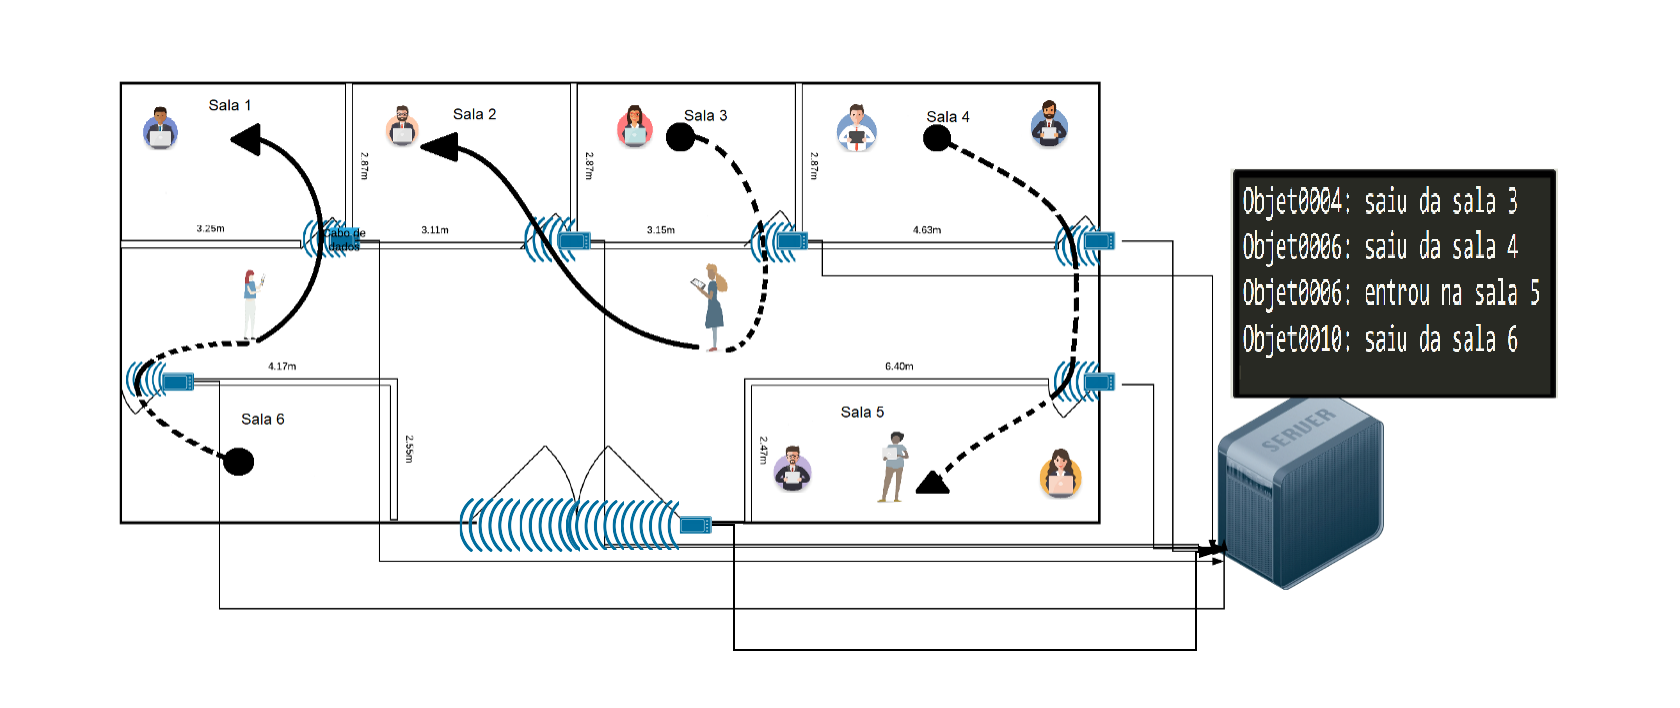
\includegraphics[width=1.1\textwidth]{Figuras/bigpicture.png}
              \legend{Fonte: Própria}
        \end{figure}

\par
Na \autoref{fig:modelo} é possível notar que há um dispositivo acoplado próximo a
porta de cada sala, esse dispositivo contém o leitor RFID e será encarregado de consultar o
servidor para assim tomar decisões do que será feito com o status do objeto, como cada objeto possui uma tag RFID fixada
nele e quando o mesmo passar pela porta o leitor identifica o objeto e altera suas informações sobre sua localização na base de dados no servidor web.

\par
O método proposto consiste nas seguintes etapas:
\begin{enumerate}
    \item Identificação dos objetos que serão rastreados;
    \item Monitoramento e localização dos objetos rastreáveis em ambiente indoor; 
    \item Configuração de controle e monitoramento de transição dos objetos; e
    \item Levantamento de todos objetos etiquetados cadastrados no sistema.
\end{enumerate}

%\todo[inline]{Aqui sugiro apresentar pelo meno um diagrama UML de caso de uso do seu sistema. Para consolidar o background das seções.}
\par
As funcionalidades do sistema e a interação com o usuário pode ser visualizada na \autoref{fig:caso_uso} e que seguem o seguinte fluxo:  as setas partindo do ator usuário até o módulo representa funções que são realizadas pelo próprio usuário do sistema; 
as setas que saem dos módulos e chegam no servidor são as operações que são solicitadas e que o servidor executa; e 
as setas que saem do servidor e chegam nos módulos representa operações que o servidor executa de forma automática.
\begin{figure}[H]
              \caption{\label{fig:caso_uso}{Caso de uso}}
              \centering
              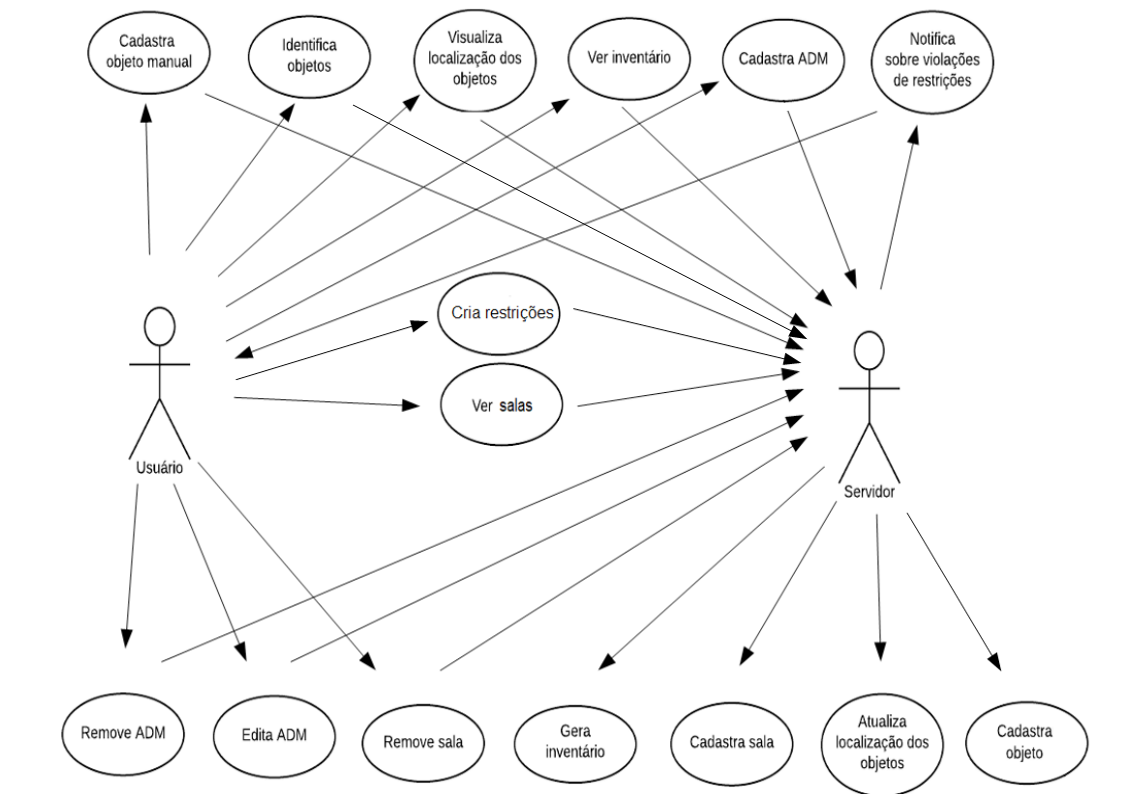
\includegraphics[width=1.1\textwidth]{Figuras/caso_de_uso.png}
              \legend{Fonte: Própria}
        \end{figure}
%
%
\section{Identificação dos objetos rastreáveis}

%Antes de qualquer passo, e visando a implantação do sistema proposto, é necessário a identificação dos objetos.
%Nessa etapa são anexado ao objetos as etiquetas RFID e realizada uma descrição do objeto portador dessa etiqueta
%no sistema, para que ao entrar e sair das salas do edifício além de fornecer a localização do objeto também seja
%possível ter detalhes sobre aquele objeto, dessa forma se objeto tiver uma registro local isso irá constar na
%descrição do objeto. Essa etapa pode ser considerada como a fase de cadastro do objeto.
Esta etapa consiste na identificação dos objetos. Primeiramente, as etiquetas RFID passiva são anexadas em cada objeto, essas etiquetas trabalham na frequência $13,56MHz$, um exemplo de objeto com uma etiqueta anexada em seu corpo pode ser visto na \autoref{fig:objeto}.
\begin{figure}[H]
              \caption{\label{fig:objeto}{Objeto com tag RFID}}
              \centering
              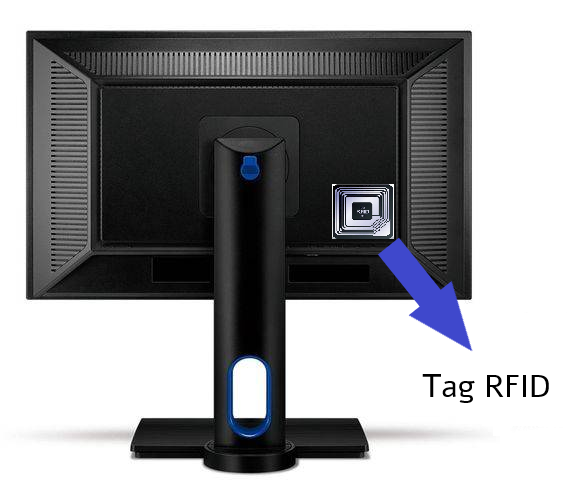
\includegraphics[width=0.4\textwidth]{Figuras/monitor.png}
              \legend{Fonte: Própria}
\end{figure}

\par
%Na \autoref{fig:objeto} é apresentado um objeto com uma tag RFID passiva anexada em seu corpo, todos os objetos que serão rastreáveis no sistemas possuirão uma tag RFID anexada da mesma forma.
%\todo[inline]{Sugiro adicionar um texto e uma descrição sobre as etiquetas RFID, bem como, as que são utilizadas no sistema.}
O segundo passo é realizar o cadastramento dos objetos utilizando algum dispositivo de porta, fazemos com que o dispositivo faça a leitura da tag do objeto, dessa forma o sistema realizará o cadastro da etiqueta porém todas as informações referente aquela etiqueta irão constar no sistema como \textbf{Desconhecido}, assim como a \autoref{fig:tela_inical} mostra. Vale ressaltar que para facilitar este processo de cadastro, as etiquetas RFID podem ser previamente castradas no sistema com o auxilio do dispositivo de porta, sem a necessidade de ter o objeto presente, para então em outro momento apenas efetuar a adição das etiquetas.

% print da tela inicial com novo objeto
\begin{figure}[H]
              \caption{\label{fig:tela_inical}Tela inicial}
              \centering
              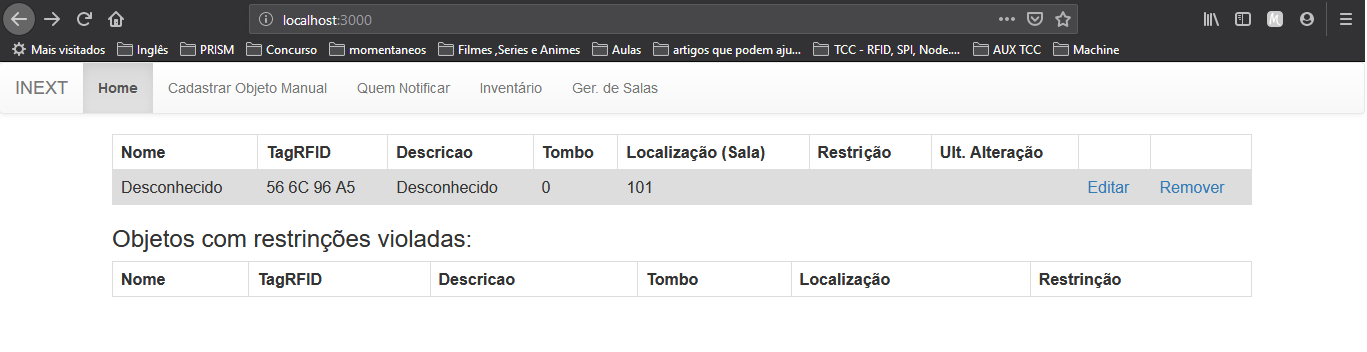
\includegraphics[width=0.9\textwidth]{Figuras/tela_inical.PNG}
              \legend{Fonte: Própria}
\end{figure}

%\todo[inline, color=green]{Sugiro ajustar o espaço entre a figura a acima e a legenda.}

\par
Durante o cadastro dos objetos, o próximo passo é editar as informações de acordo com o objeto que constam como desconhecido no sistema. Na pagina inicial é listado todos objetos cadastrados e ao lado de cada objeto possui a opção \textbf{Editar} (ver \autoref{fig:objeto}), localizamos o objeto que acabamos de realizar seu cadastro e selecionamos a opção de editar, logo seremos redirecionado para a pagina de edição de objeto e preenchemos o formulário de acordo com as características refente ao objeto desejado, após ter preenchido é necessário clicar no botão \textbf{Salvar} ao final do formulário, conforme \autoref{fig:tela_editar}.  

% print da tela editar objeto
\begin{figure}[H]
              \caption{\label{fig:tela_editar}Tela para editar objeto }
              \centering
              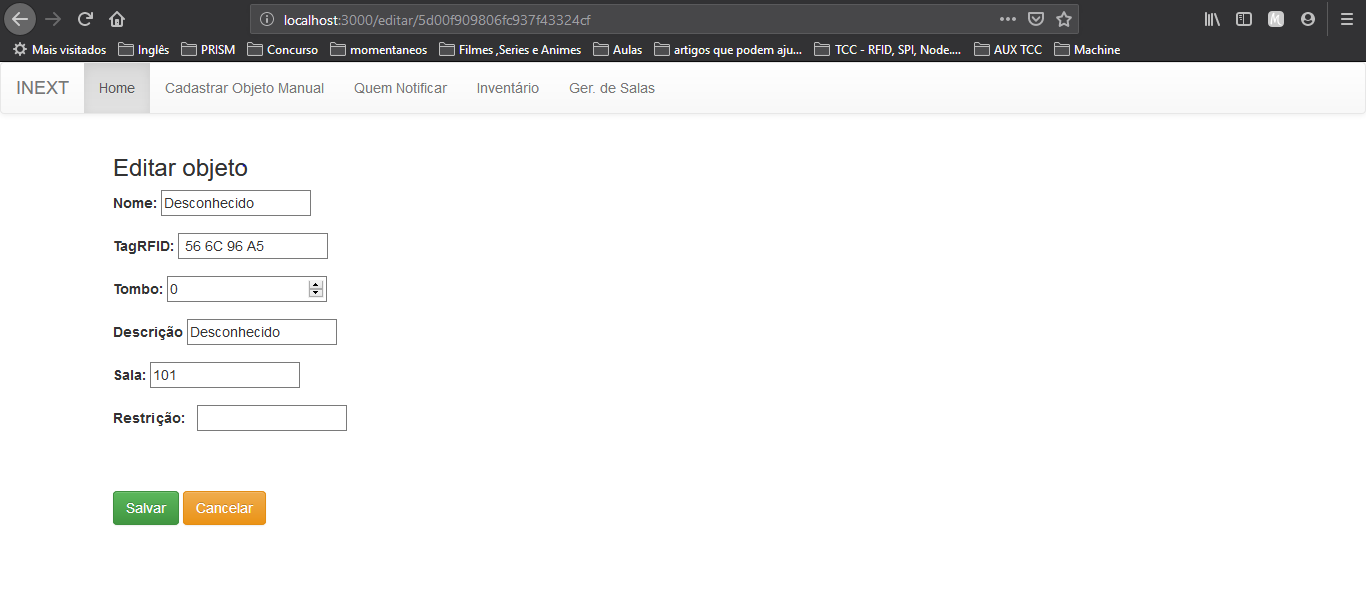
\includegraphics[width=0.9\textwidth]{Figuras/tela_editar.png}
              \legend{Fonte: Própria}
\end{figure}


\section{Monitoramento e Localização dos objetos rastreáveis}

%O monitoramento é realizado pelo sensor de RFID que estará em cada porta das salas do prédio, que é responsável
%identificar o objeto e repassar esta informação ao módulo wireless que irá enviar para um servidor web sobre as
%ocorrências/transições das salas. Assim, criando um log sobre transição de cada objeto, provendo ao usuário do sistema
%alertas para que decisões necessárias sejam tomadas.
O monitoramento é realizado pelo módulo de porta contido em cada sala do edifício, tal módulo será descrito nas seções seguintes. No momento em que um objeto é identificado por um módulo de porta de uma sala e esse objeto tem suas informações atualizadas, significa que o objeto em questão está executando uma ação de entrada ou saída de alguma sala então o servidor deve atualizar seu status de localização.


\subsection{Fluxo de execução do método em cada sala}

O dispositivo de cada sala executa o seguinte fluxo de execução para monitoramento dos objetos da sala, conforme \autoref{fig:fluxograma}. 
% O fluxo exemplifica as tarefas que cada dispositivo executará. 
No fluxograma da figura, os retângulos representam processos e os retângulos com bordas duplas processos pré-definidos, os losangos representam as tomadas de decisões,
os ícones com bordas curvas para o mesmo lado representam operações nos dados do sistema e o ícone com bordas curvas
opostas representam o início do fluxo.

\begin{figure}[H]
              \caption{\label{fig:fluxograma}{Fluxograma de cada sala}}
              \centering
              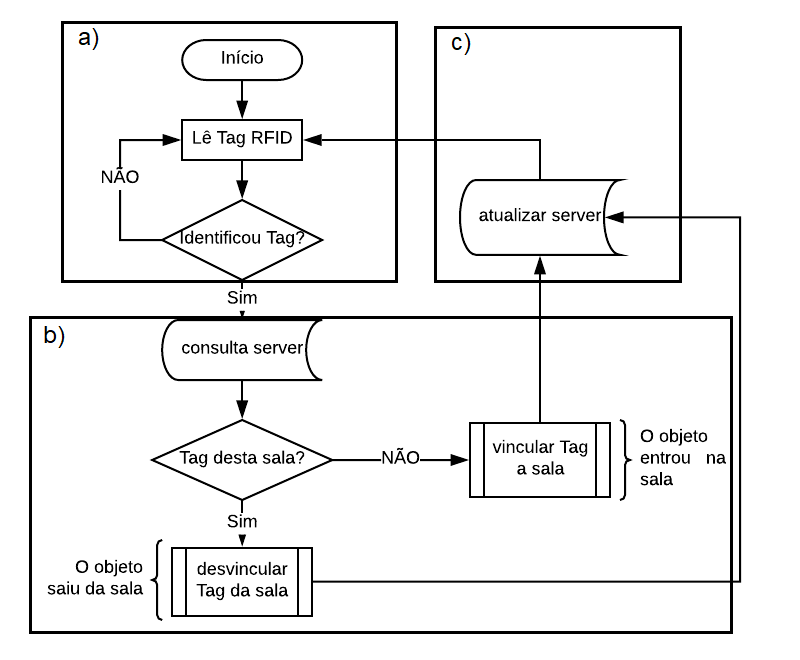
\includegraphics[width=0.7\textwidth]{Figuras/fluxograma.png}
              \legend{Fonte: Própria}
\end{figure}

\par
O fluxograma é separado em três módulos: \textbf{a}, \textbf{b} e \textbf{c}. O módulo \textbf{a} é onde é realizado o
monitoramento da da sala, realizando leituras dos objetos que entram e saem da sala. No módulo \textbf{b} é o onde são
tomadas as decisões referente a etiqueta anexada ao objeto lida naquele momento, verificando se a etiqueta está ou não
localizada naquela sala e processando as alterações necessárias. O módulo \textbf{c} é o último processo que atualiza as
informações do servidor para que os dados consultados sejam salvos e criado os logs.


\subsection{Localização dos objetos}

Os objetos são localizado no sistema baseado no algoritmo de proximidade \cite{rfid2009review} %\todo[color=green]{Adicionar referência}
, ou seja, a partir do momento em que o leitor
RFID identifica uma etiqueta, esse objeto terá ou deixará de ter a localização referente àquele módulo de porta, cada módulo representa uma sala, portanto as informações referente a localização dos objetos são definidas de acordo com o dispositivo que executa a leitura da etiqueta anexada ao objeto.

%\todo[color=green]{Sugiro descrever mais sobre este servidor web, exemplo de conexão local ou não, banco de dados e
%outras informações necessárias}
\par
O sistema possui um servidor web que para este trabalho foi desenvolvido utilizando o framework Node.js $v10.15$ disponível pra download em \url{https://nodejs.org/en/download/}%\todo[color=green]{adicionar link e versão}
, que deve está conectado à mesma rede LAN (\textit{local area network}) que os dispositivos de porta. O servidor web também possui uma base de dados, sendo o sistema de gerenciamento de dados o MongoDB $v3.6.5$ disponível em \url{https://www.mongodb.com/download-center/community}%\todo[color=green]{adicionar link e versão utilizada}
, para armazenar informações e a descrição e informações de cada objeto. Logo, o servidor web é responsável por tratar problemas relacionados as leituras das  etiquetas, também sendo responsável por realizar a levantamento do inventário total e notificar os usuários sobre violações.

\par
O Node.js e MongoDB foram as tecnologias escolhidas, pois fornece facilidades no desenvolvimento do \textit{front-end, back-end} e operações com o banco de dados utilizando apenas uma linguagem de programação que é o JavaScript, o custo de hardware dessas tecnologias é baixo viabilizando ainda mais a implementação e pode ser realizado o \textit{deploy} para outro sistema operacional com facilidade.
%\todo[inline, color=green]{Descrever o motivo pelo qual foi escolhido o Node.js e MongoDB, quais as vantagens para o sistema proposto}

%\todo[inline, color=green]{Sugiro apresentar uma imagem que represente o esquema de conexão da rede dos nós de rede das portas, pontos de acesso até o servidor.}

\begin{figure}[H]
              \caption{\label{fig:representacao_rede}{Representação da rede}}
              \centering
              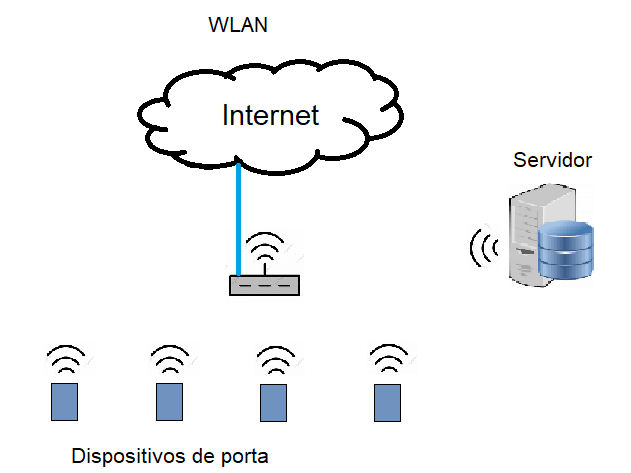
\includegraphics[width=0.7\textwidth]{Figuras/rede.png}
              \legend{Fonte: Própria}
\end{figure}

%o papel do servidor é de grande importância também sendo utilizado para consultar informações referentes aos objetos.


\section{Configuração de controle e monitoramento de transição dos objetos}

% Para um melhor gerenciamento dos objetos, o sistema conta com alertas para que caso um objeto inicie uma transição para outra sala e nesse trajeto o objeto não entre em nenhuma sala excedendo um tempo determinado, um alerta é gerado informado que o objeto não entrou em nenhuma sala do edifício até o momento da geração do alerta.

%\par
% Um tempo padrão deve ser configurado para os alertas, se um objeto exceder esse tempo na transição um alerta é gerado no servidor. O tempo deve ser configurado na implantação do sistema. Um outro alerta que pode ser criado seria no caso de ser definido uma área de limite para alguns objetos e ele sejam deslocados para fora dessa área delimitada.
\par 
Visando um melhor gerenciamento e rastreamento dos objetos no sistema proposto, todas as operações do sistema geram logs. Os arquivos contendo os logs são criados diariamente e os nomes desses arquivos são de acordo com a data, por exemplo, um log do dia 07 de junho de 2019 tem como seu nome a data \texttt{2019-06-07}. Um arquivo de log pode ser visualizado na \autoref{fig:tela_log}, no canto superior esquerdo da imagem tem o nome do arquivo e no seu corpo tem algumas das operações que ocorreram.

\begin{figure}[H]
              \caption{\label{fig:tela_log}Arquivo de log}
              \centering
              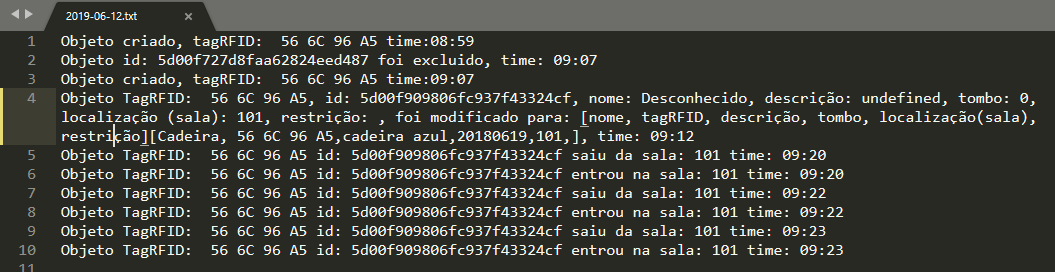
\includegraphics[width=1\textwidth]{Figuras/tela_logs.png}
              \legend{Fonte: Própria}
\end{figure}
\par
%Cada transição de objeto também é armazenada nos logs do sistema com data e hora, sala que saiu ou entrou, para que os eventos ocorridos sejam registrados e possua mais um recurso na consulta para caso ocorram falhas.
%\todo[inline,color=green]{Sugiro descrever um pouco mais, talvez falar que com os dados de log das
%transições do sistema é possível também delimitar
%salas que objetos não podem sair, ou não podem entrar, criando zonas de controle.}
O sistema também conta a opção de definir restrições aos objetos monitorados, exemplo, um objeto que no campo de restrição tem o nome de uma sala, ao sair dessa sala o sistema identifica esta violação de condição e comunica os administradores enviando um e-mail com os dados do objeto que violou a restrição. Na \autoref{fig:tela_restricao} é mostrado como o objeto com restrição é mostrado no sistema e o e-mail enviado. Essa função é importante para objetos que não podem ser levados para outras salas, tendo que permanecer em uma única sala. 
%\todo[inline, color=green]{Sugiro adicionar um texto descrevendo a importância desta opção do sistema}
\begin{figure}[H]
              \caption{\label{fig:tela_restricao}Restrição}
              \centering
              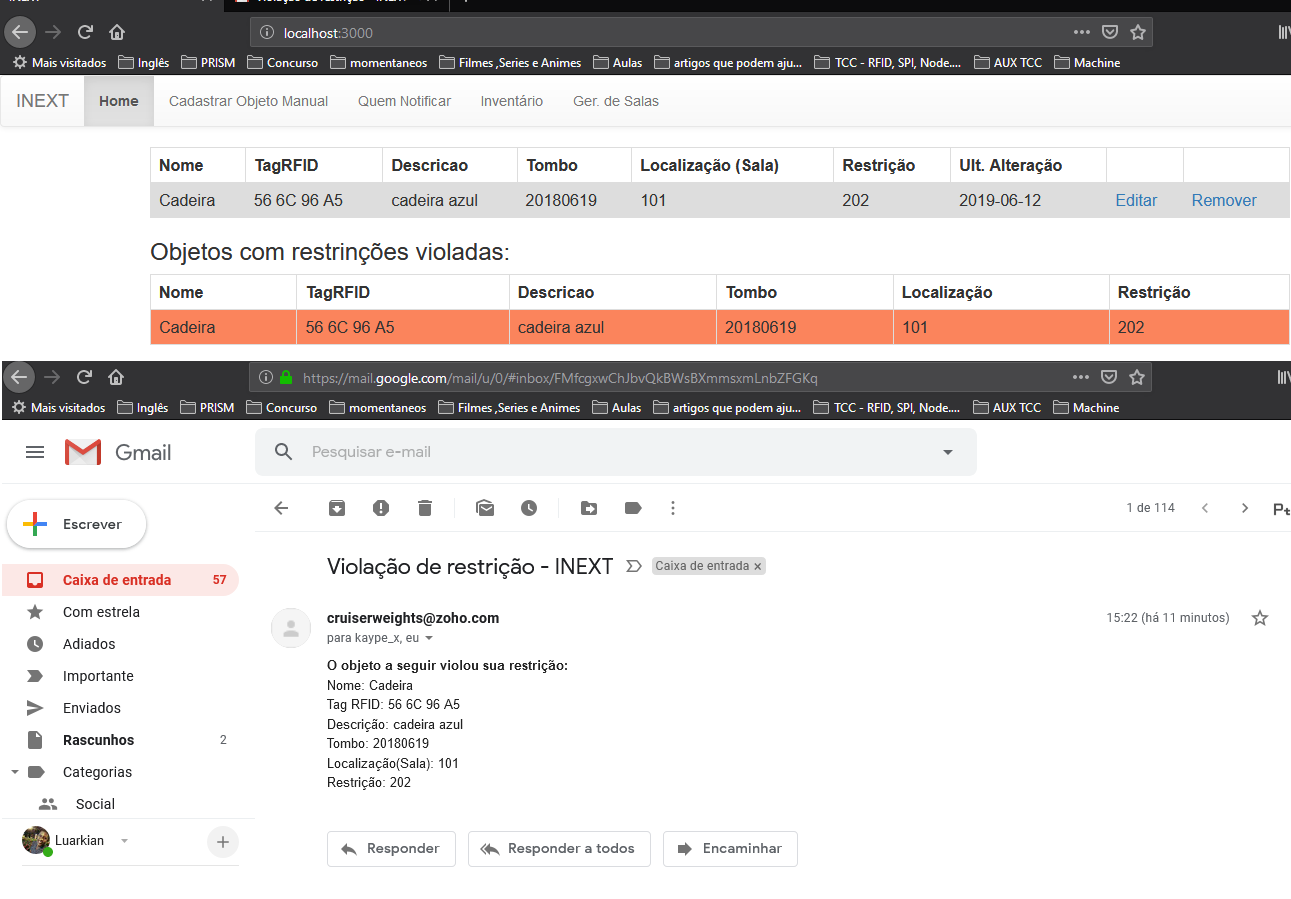
\includegraphics[width=1\textwidth]{Figuras/tela_restricao.png}
              \legend{Fonte: Própria}
\end{figure}


\section{Conexão dos dispositivos de porta com o servidor}

A comunicação no sistema entre os dispositivos da porta com o servidor web acontece por meio de uma WLAN, ou seja todos devem estar em uma rede local e assim poderem se comunicar, entretanto a comunicação será diretamente entre um dispositivo e o servidor,
não havendo comunicação entre dois dispositivos. Neste trabalho, foi utilizado a placa NodeMcu ESP-12E, \textit{datasheet} disponível em \url{https://www.electrodragon.com/w/ESP-12F_ESP8266_Wifi_Board}, %\todo[color=green]{link e versão utilizada} 
que possui um módulo ESP-8266, esse módulo possibilita a conexão com uma rede wireless 802.11 b/g/n, esse padrão possibilita conexões com velocidade de até $300Mbps$ em um espectro de $2.4GHz$ ou $5GHz$. % \todo[color=green]{descrever as vantagens deste tipo de conexão}.
%\todo[color=green]{Falar um pouco sobre baixo consumo de energia}.

\par
Os dispositivos de porta, ao realizar a leitura de um etiqueta, geram um objeto JSON (\textit{JavaScript Object Notation}), esse objeto contém o nome da sala e o identificado da tag RFID, depois de criado o objeto é enviado para o servidor via requisição POST para executar as operações e modificar o status do objeto que esta com a etiqueta anexada.
%\todo[inline, color=green]{Apresentar um exemplo de JSON gerado}

% [H][style=json]
\begin{lstlisting}[language=json,firstnumber=1]
// Exemplo de um JSON gerado
{
    "sala": "101",
    "tagRFID": " 56 6C 96 A5"
}  
\end{lstlisting}

\par
O NodeMcu opera em uma voltagem de $5$V de energia contínua, um consumo relativamente baixo em relação as outros dispositivos eletrônicos e as etiquetas passivas não possuem alimentação, elas são alimentadas apenas pela energia eletromagnética emitida pelos leitores RFID, esses dois quesitos tornam o protótipo ainda mais viável, pois isso é um fator positivo visto que o custo pós implantação não é alto em relação ao consumo de energia.

%\todo[inline,color=green]{Sugiro descrever como seria a possibilidade de usar os dispositivos de porta com uma bateria de 9v e qual o tempo de duração (vai ficar para trabalhos futuros)}


\section{Dispositivos de porta}

O protótipo desenvolvido neste trabalho comumente chamado de dispositivo da porta, é composto por uma placa NodeMcu e um leitor RFID RC522 Mifare, \textit{datasheet} disponível em \url{https://www.nxp.com/docs/en/data-sheet/MFRC522.pdf}.  %\todo[color= green]{link e versão}
O leitor RFID pode ser visto na \autoref{fig:leitorRFID}, esse leitor é capaz de ler etiquetas que operam em
frequências de $13,56MHz$. 
% 
Vale ressaltar que o protótipo visa avaliar a aplicabilidade do sistema proposto, visto que o leitor RFID pode ser facilmente substituído por outro de maior alcance de leitura das etiquetas.
% 
O código para o NodeMcu se encontra no repositório do GiHub \url{https://github.com/luarkian/nodeArd-INEXT.git} dentro da pasta \texttt{prototype\_nodemcu} e antes de embarcar o código deve ser colocado o endereço IP do servidor web na variável \texttt{url}.
\begin{figure}[H]
              \caption{\label{fig:leitorRFID}{Leitor RFID RC522}}
              \centering
              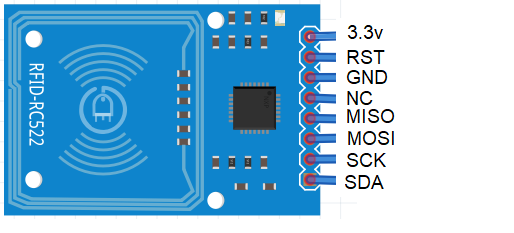
\includegraphics[width=0.7\textwidth]{Figuras/rfid_rc522.PNG}
              \legend{Fonte: Fritzing}
\end{figure}

\par
O leitor RFID utiliza a interface SPI (\textit{Serial Peripheral Interface} ) para comunicação com o NodeMcu,
essa conexão é síncrona e é realizada por meio dos pinos de \textbf{D2, D4, D5, D6} e \textbf{D7}. A prototipagem entre o NodeMcu e o leitor RFID
segue o esquema na \autoref{fig:esq_conexoes}:

\begin{itemize}
    \item 3.3V - conectado ao pino de 3.3v no NodeMcu, essa conexão faz a alimentação do leitor RFID;
    \item RST (\textit{Reset})- conectado ao pino D2 do Arduíno;
    \item GND (\textit{Graduated Neutral Density filter}) - conectado ao pino GND do NodeMcu;
    \item NC/IRQ (\textit{Interrupt Request})- não utilizado;
    \item MISO (\textit{Master In Slave Out}) - conectado ao pino D6;
    \item MOSI  (\textit{Master Out Slave In}) - conectado ao pino D7;
    \item SCK  (\textit{Serial Clock}) - conectado ao pino D5; e
    \item SDA/SS (\textit{Serial Data Line/ Select Slave}) - conectado ao pino D4.
\end{itemize}

\begin{figure}[H]
              \caption{\label{fig:esq_conexoes}{Esquema de Conexões}}
              \centering
              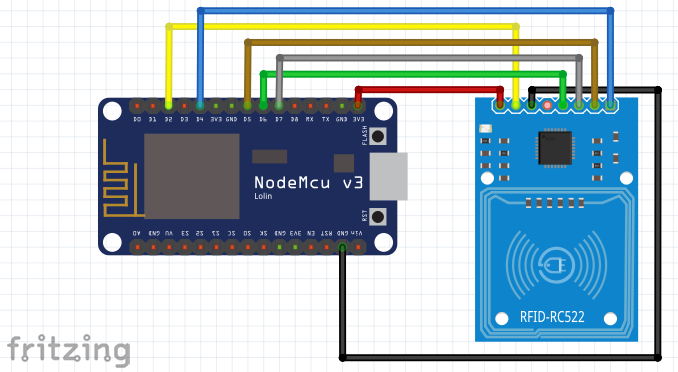
\includegraphics[width=1\textwidth]{Figuras/esquema_nodemcu_rc522.PNG}
              \legend{Fonte: Própria}
\end{figure}

\begin{comment}

\begin{figure}[H]
              \caption{\label{fig:moduloWii}{Módulo Wifi ESP8266}}
              \centering
              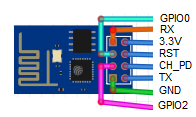
\includegraphics[width=0.6\textwidth]{Figuras/Modulo_ESP8266.png}
              \legend{Fonte: Fritzing}
\end{figure}

\par
O ESP8266 é um módulo que permite a conexão do Arduíno com redes wireless 802.11 b/g/n, esse módulo pode
trabalhar em dois modos tanto como ponto de acesso ou no modo estação que envia e recebe dados.
%\todo[color=green]{Descrever}.

\begin{itemize}
    \item GND (\textit{graduated neutral density filter}) - conectado ao pino GND do Arduíno;
    \item GPIO0 (\textit{General Purpose Input/Output}) - não conectado ;
    \item GPIO2 (\textit{General Purpose Input/Output})- não conectado ;
    \item TX (\textit{Transmission}) - conectado ao pino digital 2 no Arduíno;
    \item RX (\textit{Received})- conectado ao pino digital 3 no Arduíno junto com dois resistores um de 220$\Omega$ e outro de 330$\Omega$ para dividir a tensão;
    \item RST (\textit{Reset}) - não conectado ;
    \item CH\_PD (\textit{Chip enable}) - conectado ao pino 3.3v mas com resistor de 10 $K\Omega$.
\end{itemize}
\end{comment}
%\todo[inline,color=green]{Descrever a função dos pinos}

%\begin{figure}[H]
%              \caption{\label{fig:esq_conexoes}{Esquema de Conexões}}
%              \centering
%              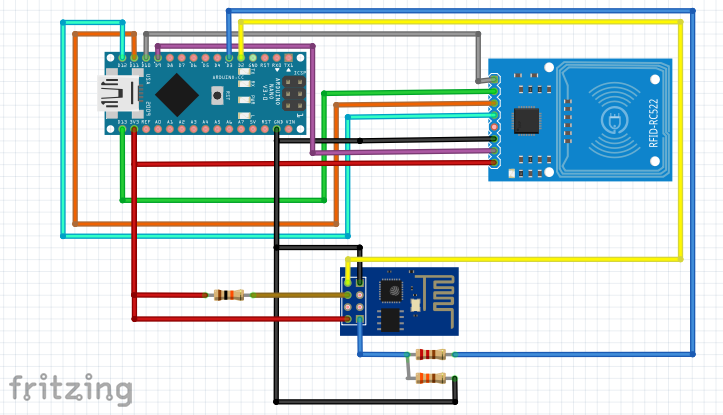
\includegraphics[width=1\textwidth]{Figuras/esquema_de_conexoes2.PNG}
%              \legend{Fonte: Própria}
%\end{figure}

\section{Servidor Web}

O servidor web foi desenvolvido utilizando a tecnologia Node.js $v10.15$ utilizando a linguagem de programação JavaScript e o sistema de gerenciamento de banco de dados orientado a documento MongoDB $v3.6.5$. Através do Node.js e seu gerenciado de pacotes NPM foram instaladas as seguintes bibliotecas e suas respectivas versões. Todas as bibliotecas instaladas podem ser encontradas nas dependências no arquivo \textit{package.json} que se encontra no repositório deste trabalho. 

\begin{itemize}
    \item Express $v4.16.4$ - foi utilizada para criar as rotas e instanciar o serviço HTTP;
    \item Express-ejs-layouts $v2.5$ - foi utilizada pra acessar as \textit{views}; 
    \item Mongoose $v3.1.13$ - foi utilizada para modelar os objetos;
    \item Nodemailer $v6.1.1$ - foi utilizado para o envio de e-mails a partir da aplicação;
    \item EJS $v2.6.1$ - foi utilizada para a criação de \textit{views} do \textit{front-end};
    \item Consign $v0.1.6$ - foi utilizado para realizar o carregamento de \textit{scripts} automaticamente;
    \item Moment $v2.24$ - foi utilizada para a manipulação de datas e hora.
\end{itemize}

%\todo[inline, color=green]{Descrever a função de cada biblioteca utilizada}


% A seguir as bibliotecas foram instaladas mais não foram utilizadas:

% \begin{itemize}
%     \item Serialport $v7.1.4$
%     \item Socket.io $v2.2.0$
%     \item Socket.io-client $v2.2.0$
% \end{itemize}

\par 
O sistema do servidor web possui as seguintes telas: 
% que podem ser vitas no \autoref{chapter:anexo} ANEXO A:%\todo[color=green]{Criar anexo} 
\begin{itemize}
    \item Tela Inicial
    \item Tela de Cadastro de Objeto Manual
    \item Tela de Editar Objeto
    \item Tela de Quem Notificar
    \item Tela de Editar ADM
    \item Tela de Inventário
    \item Tela de Ger. Sala
\end{itemize}    

%\todo[inline]{Sugiro apresentar o storyboard do fluxo entre as telas.}

%\todo[inline, color=green]{Mover estas telas para um Anexo}

\subsection{Implementação}

% Os códigos foram escritos utilizando o editor de texto \textit{Sublime Text} na versão 3.2.1 
Na codificação do sistema foi utiliza a linguagem de programação JavaScript no \textit{back-end} e \textit{front-end}, a linguagem de marcação HTML(\textit{HyperText Markup Language}) para construção das telas e mecanismo CSS (\textit{Cascading Style Sheets}) para modificar o estilo das páginas web, sendo que alguns estilos são fornecidos pelo framework \textit{Bootstrap} $v3.3.4$ disponível em \url{http://getbootstrap.com}.

\subsubsection{\textit{Back-End}}

O \textit{Back-End} deste sistema possui a estrutura mostrado na \autoref{fig:backend}.
\begin{figure}[H]
	  \caption{\label{fig:backend}Arquivos do Back-end}
	  \centering
	  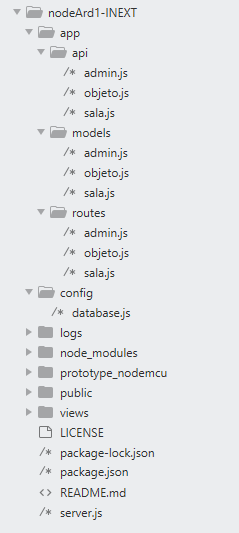
\includegraphics[width=0.3\textwidth]{Figuras/back_end.PNG}
	  \legend{Fonte: Própria}
\end{figure}
    
\par 
Na pasta \textit{config} possui o arquivo  \texttt{database.js}, é neste arquivo em que estão as configurações do mongoose para realizar a conexão com o MongoDB. 
% \par
Dentro da pasta  \textbf{app} há mais três pastas: api, models e routes. 
% Nessas pastas tem três arquivos com os nomes \textit{admin.js}, \textit{objeto.js} e \textit{sala.js}. 
Os arquivos dentro da pasta \textbf{models} são para descrever os campos que os objetos JSON devem ter para serem salvos e manipulados no sistema.
% \par
% O objeto ''admin'' possui dois campos: ''nome'' e ''email'', os objetos ''salas'', também possui dois campos: ''nome'' e ''bloco'' porém o campo ''bloco'' ainda não está como obrigatório e pode ser deixado em branco e os objetos rastreáveis possuem os campos: ''nome'',''tagRFID'', ''tombo'', ''sala'', ''restricao'', ''alerta'' e ''alteracao''.
% \par
Na pasta \textbf{api} estão os aquivos com módulos que executam as operações do sistema e na pasta \textbf{routes} é onde são implementos os caminhos para acessar os módulos da pasta \textbf{api}. Assim como na pasta \textbf{models} as pastas \textbf{api} e \textbf{routes} também possuem cada uma os arquivos com os nomes \texttt{admin.js}, \texttt{objeto.js} e \texttt{sala.js}, porém os conteúdos dos arquivos contém a implementação dos módulos e dos caminhos.

\par
Módulos dos arquivos \texttt{admin.js} contidos nas pastas \textbf{api} e \textbf{routes}.
\begin{itemize}
    \item \texttt{/admin/}, \texttt{api.lista}:  rota e módulo que retornam todos os usuários cadastrados através de uma requisição GET;

    \item \texttt{/admin\_dados}, \texttt{api.criar}: rota e módulo para cadastrar administradores no sistema, deve ser enviado um JSON via requisição POST;
    
    \item \texttt{/admin\_edit/:id}, \texttt{api.buscarPorId}: rota e módulo que retorna ao administrador que for informado o \texttt{ID} na URL, é uma requisição GET;
    
    \item \texttt{/editarAdm/:id}, \texttt{api.atualizaDados}: rota e módulo para atualizar dados do administrador que for informado o \texttt{ID} na URL e um objeto JSON dever ser enviado com as novas informações via requisição POST; e
    
    \item \texttt{/removeAdm/:id} , \texttt{api.removePorId}: rota e módulo para exclusão do administrador que for informado o \texttt{ID} na URL, é uma requisição GET.
\end{itemize}


\par
Módulos dos arquivos \texttt{sala.js} contidos nas pastas \textbf{api} e \textbf{routes}
\begin{itemize}
    \item \texttt{/sala/}, \texttt{api.listar}: essa rota juntamente com esse modulo retornar as lista de todas as sala cadastradas, é uma requisição GET; e

    \item \texttt{/removeSala/:id}, \texttt{api.excluir}: essa rota e módulo excluem a sala cujo o \texttt{ID} é passado na URL, é uma requisição GET;
\end{itemize}


\par
Módulos dos arquivos \texttt{objeto.js} contidos nas pastas \textbf{api} e \textbf{routes}
\begin{itemize}
    \item  \texttt{/}: essa rota não possui um módulo, seu módulo foi implementado no próprio arquivo de rotas, é uma requisição GET e retorna todos os objetos cadastrados no banco de dados;

    \item \texttt{/cadastrar}, \texttt{api.adiciona}: rota e módulo para cadastrar objeto no sistema, deve ser enviado um JSON via requisição POST;

    \item \texttt{/objetos}, \texttt{api.lista}: rota e módulo que retornam todos os objetos cadastrados através de uma requisição GET;

    \item \texttt{/verificacao}, \texttt{api.verificar}: rota e módulo que executa as operações de transições dos objetos, cria alertas e envia e-mail para os administradores, deve ser enviado um JSON via requisição POST;

    \item \texttt{/ver}, \texttt{api.ver}: rota e módulo destinada a teste para imprimir os JSON's recebidos no console, deve ser enviado um JSON via requisição POST;

    \item \texttt{/editar/:id}, \texttt{api.buscaId}: rota e módulo que retorna o  objeto que for informado o ID na URL, é uma requisição GET;

    \item \texttt{/editar/:id}, \texttt{api.atualizar}: rota e módulo para atualizar dados do objeto que for informado o ID na URL e um objeto JSON dever ser enviado com as novas informações via requisição POST;

    \item \texttt{/remove/:id}, \texttt{api.removePorId}: essa rota e módulo excluem o objeto cujo o ID é passado na URL, é uma requisição GET; e
    
    \item \texttt{/inventario}, \texttt{api.inventario}: rota e módulo que retornam todos os objetos e salas cadastrados através de uma requisição GET.

\end{itemize}

\par 
O arquivo \texttt{server.js} na raiz do diretório é responsável por importar todos os arquivos mencionados anteriormente e iniciar o serviço \textit{HTTP} na porta $3000$. É importante ressaltar que antes de qualquer rota deve ser colocado o endereço IP que o servidor possui na rede WLAN.

%\todo[inline]{(Está descrito nos Resultados )Seria interessante adicionar uma seção descrevendo os cenários do uso para o levantamento de patrimônio e relação ao da UFRR}